\chapter{The EM algorithm and Information Theory}

\section{Mixture Models}\label{sec:mixtureModels}

In the previous chapter we have mentioned that it may happen that a likelihood function has multiple 
maxima and that sometimes it may be hard to impossible to find the global maximum (i.e.\ the maximum
with the overall highest likelihood value). Such a situation occurs whenever the probabilistic model
that we use to model our observations is a \textbf{mixture model}.

\begin{Definition}[Mixture Model]\label{def:mixtureModel}
Given any set of probability distributions $ P_{X_1}, \ldots, P_{X_n} $ \chris{that are defined over the same
random variable $ X $??? over the same probability space?... leave it out?} we define a mixture model as
$ P = \underset{i=1}{\overset{n}{\sum}} \alpha_{i}P_{X_i} $
where we require that all $ \alpha_{i} \geq 0$ and 
$ \underset{i=1}{\overset{n}{\sum}} \alpha_{i} = 1 $.
We call the distributions $ P_{X_1}, \ldots, P_{X_n} $ \textbf{mixture components} and their weights
$ \alpha_{i} $ \textbf{mixture weights}.
\end{Definition}

Mixture models are extremely useful whenever we have different ways to think about our data. Each way
of conceptualising our data can be encoded by one of the mixture components of the mixture model.
This point of view can help us to build a better overall model of our data. Let us introduce a running example that
we use for the rest of this section. 

\paragraph{Example of a mixture model} Assume we observe 10 sequences of coin tosses. Each sequence
contains 100\chris{might be less confusing to choose two different numbers for the number of sequences and number of coin flips per sequence} flips. We also know that there are 3 coins with which these sequences could possibly be
generated and for each sequence a different coin may have been used. Coin 1 is unbiased, coin 2 has
parameter $ \theta = 0.3 $ and coin 3 has parameter $ \theta = 0.65 $. 
 
We could use 
a multinomial distribution over coins to model our data. We would then employ maximum likelihood estimation 
and pick the coin that has the highest likelihood \chris{per sequence? This is my general problem with this running example. What are we looking for exactly???}. However, this model might actually turn out to be
pretty bad because we are committing to picking only one coin, although we said in the beginning that
each sequence may possibly have been generated by a different coin. 

A mixture model comes to the rescue. Instead of assuming that only one coin has generated all 10 sequences,
we assume that all three coins have contributed to generating the 10 sequences. However, their distributions
may not be equal. This inequality is exactly what the mixture weights capture. As usual, we call our data $ x $. Also, each mixture component is a binomial distribution, parametrized by the parameters of
the coins. These observations suffice to formulate our mixture model.
\begin{align}\label{eq:mixtureExample}
&P(X=x|\Theta_{1}^{3}=\theta_{1}^{3}, A = \alpha_{1}^{3}) 
= \alpha_{1}P(X=x|\Theta_{1}=0.4) \\
&+ \alpha_{2}P(X=x|\Theta_{2}=0.5) + \alpha_{3}P(X=x|\Theta_{3}=0.65) \nonumber
\end{align}

Notice that if we were given the mixture weights, estimating
the parameters of the mixture components would be easy: we would simply find the MLE for each mixture component. The mixture
model could then easily be constructed because the mixture weights are known. 

What happens if both the parameters of the mixture components and the mixture weights are unknown? First, observe the constraints
on mixture weights in Definition~\ref{def:mixtureModel}. All mixture weights have to be non-negative and they have to sum to 1.
These constraints mean that we can interpret the weights as a probability distribution. In particular, the weights form a distribution over parameters
of the mixture components (assuming that all mixture components have the same parametric form). That is, we get the following
relations:
\begin{equation}
\hskip 0.5cm \alpha_{1} = P(\Theta_{1} = \theta_{1}) \hskip 0.5cm \alpha_{2} = P(\Theta_{2} = \theta_{1}) \hskip 0.5cm \alpha_{3} = P(\Theta_{3} = \theta_{1})
\end{equation}
Hence, we can rewrite our mixture model as
\begin{align} \label{eq:probabilisticMixtureModel}
&P(X=x) 
= P(\Theta_{1} = 0.4)P(X=x|\Theta_{1}=0.4) \\
&+ P(\Theta_{2} = 0.5)P(X=x|\Theta_{2}=0.5) + P(\Theta_{3} = 0.65)P(X=x|\Theta_{3}=0.65) \nonumber
\end{align}

Notice that in our examples we assume that we have only three possible binomial parameters, namely $ \theta_{1} = 0.4, \theta_{2} = 0.5, \theta_{3} = 0.65 $. 
Notice further that each summand
in \eqref{eq:probabilisticMixtureModel} is in fact a joint distribution by the chain rule so that we can again rewrite the model as
\begin{align}
\begin{split}\label{eq:marginal}
P(X=x) &= P(X=x,\Theta_{1}=0.4) + P(X=x,\Theta_{2}=0.5)  \\
&\quad + P(X=x,\Theta_{3}=0.65)
\end{split} \\
&= \underset{i=1}{\overset{3}{{\sum}}} P(X=x,\Theta=\theta_{i}) \nonumber
\end{align}
where \eqref{eq:marginal} is a simple marginalisation step. Notice that we have just accomplished something impressive: we have given a probabilistic justification
for why mixture models do indeed model our data. Each mixture-component/weight pair gives rise to a joint distribution over parameters and data but by summing over the 
possible parameters we get the probability of the data. By induction, we can easily show that mixture models can be defined for any number of mixture components.

\begin{Exercise}
Show that a mixture model of size $ n $ is a model of the data, i.e.\ show that $  \sum_{i=1}^n \alpha_{i}P(X_i=x) = P(X=x) $ \chris{The previous $P_i$ was not defined} if $ \alpha_{i} $ are mixture weights as 
defined in \eqref{def:mixtureModel}.
\end{Exercise}

Notice that we have shown above that the formulation of mixture models as purely probabilistic model and as linear combinations of probability distributions are
equivalent. So why did we even bother to give a purely probabilistic justification? On the one hand, it is mathematically satisfying to trace back new concepts
to concepts that we are already familiar with (like joint distributions and the chain rule). More importantly, however, the probabilistic interpretation of mixture
weights allows us to estimate them using the maximum-likelihood principle. This estimation is something we could not have done, if we had regarded them solely as scale factors
for the mixture components. 

There is one additional problem, however: if both the mixture weights and the mixture components are unknown, there is no closed-form solution for estimating the
MLE. In other words, we can not simply apply calculus as we have been doing up to now. For this reason, we turn to the \textbf{EM algorithm}, that allows
us to at least find a local maximum of the likelihood function.


\section{The EM algorithm}

In order to estimate the parameters of mixture models, we can employ a classical algorithm of 
\textbf{unsupervised learning}, namely the \textbf{expectation-maximisation (EM) algorithm}. This
algorithm allows us to find a local maximum of the likelihood function of mixture models or, more
generally, models with missing data. 

Let us quickly introduce the idea of missing data: Assume you run a website that recommends movies
based on a user's preferences. In order to make statistical predictions about what type of user
likes what kind of movie, you ask your users to rate movies according to different categories.
Say you ask your users to rate the movies for entertainment value, action and fun. What may happen is
that some of your users only rate a movie in one or two of these three categories. However, these
ratings are still valuable to you and you do not want to throw them away, just because they are lacking
a rating in one category. Thus you have a data set with some missing data that you have to fill in somehow.

\medskip 
In mixture models, annotations that tell you which mixture component
generated a given data point can be thought of as missing data. If you had this information, you could simply do maximum likelihood estimation.
However, since you do not know which mixture component generated your data point, you can only
assume that all mixture components may have done so with a probability that is given by their mixture
weights. 

The EM algorithm allows you to probabilistically fill in the missing data and find good mixture weights
(where you should understand \textit{good} in the maximum-likelihood sense). The idea behind the
algorithm is simple: compute the expected number of occurrences of the missing data values (the mixture 
components) and then do maximum likelihood estimation on those expectations. Repeat the procedure 
until the likelihood does not increase any further. Notice that this procedure requires you to
fix the number of mixture components in advance.

More formally, assume a data set $ x_{1}^{n} $. Furthermore, define $ Y $ as a random variable indicating $ m $ possible
mixture components. In the more general case of missing data, $ Y $ is called \textbf{latent} or \textbf{hidden variable}
because it is not observed. Then the likelihood function if 
\begin{align}
L_{x}(\theta) = P(X=x|\Theta=\theta) = \underset{y=1}{\overset{m}{\sum}} P(X=x, Y=y|\Theta=\theta)
\end{align}
where $ \Theta $ ranges over the parameters of the joint distribution $ P_{XY} $. Let $ t(y) $ be any
statistic of the latent data. In most practical applications, $ t(y) $ is simply the count of the latent
value $ y $ in the latent data. Then, given some estimate $ \overline{\theta}^{(i)} $ for the parameters of the joint
distribution compute the expected value of the statistic $ t(y) $. \chris{Hmm, what is the RV in this expectation? We should have some RV to compute the expectation over... while fixing the data $x$ and the parameter $\theta$. I'm also confused about the $y$. Notation-wise it looks like an outcome of $Y$, so $y \in \supp(Y)$, but it could also be the ``latent data'' (in analogy to $x$ which is the data)? Or is it $t(Y)$ and the expectation is taken over $Y$?}
\begin{equation} \label{Estep}
t(y)^{(i+1)} = \E(t(y)|X = x,\Theta = \overline{\theta}^{(i+1)})
\end{equation} 
\chris{should it be conditioned on $\theta^{(i)}$?}

Observe that we introduced superscripts.\chris{and why the overline of $\theta$?} The EM algorithm is an iterative algorithm, meaning we repeat its steps several
times. We use the the superscript to indicate the number $i$ of the repetition, thus $ 0 \leq i \leq m $. We percolate \chris{what's that?}
information from previous iterations by conditioning on their parameter estimates; $ \overline{\theta}^{(0)} $ can be set arbitrarily.

Equation~\eqref{Estep} is know as the \textbf{E(xpectation)-step} of the EM algorithm. To make the algorithm complete, we are still lacking a
\textbf{M(aximization)-step}. But that step is simple. We pretend that the expected statistics of the latent data were actually observed. If
our statistics are counts, then we simply pretend that we observed outcome $ y $ exactly $ t(y)^{(i+1)} $ times. Notice that since $ t(y)^{(i+1)} $
is an expectation, it is a real and not a natural number. Once we pretend to observe the expected statistics, the maximization step can be done
using be maximum-likelihood estimation:
\begin{equation} \label{Mstep}
\overline{\theta}^{(i+1)} = \underset{\theta}{\arg\max} P(X=x, t(Y) = t(y)|\theta)
\end{equation}

\begin{Definition}[EM algorithm]\label{def:EM}
We assume a data set $ x = x_{1}^{n} $ and postulate that there is unobserved data $ y = y_{1}^{m} $ that belongs to that data set. We also
assume a probabilistic model whose parameters are realisations of a RV $ \Theta $. Take any
statistic $ t(y) $ of the latent data. Then any iterative algorithm with $ k $ iterations that performs the following steps for $0\leq i \leq k$,
\begin{align*}
\mbox{\textbf{E-step:} } \quad t(y)^{(i+1)} &= \E(t(y) \mid X = x, \Theta = \overline{\theta}^{(i+1)}) \\
\mbox{\textbf{M-step:} } \qquad \overline{\theta}^{(i+1)} &= \underset{\theta}{\arg\max} \; P(X=x, t(Y) = t(y) \mid \Theta = \theta) 
\end{align*}
to update the model parameters is called an EM algorithm.
\end{Definition}

\paragraph{Example of an EM algorithm} Assume as in Section~\ref{sec:mixtureModels} that our data is $ x=x^{10}_{1} $ where each $ x_{i} $ is the 
number of heads that we observed in a sequence of a hundred coin tosses. Again we also assume mixture components that are binomials with parameters
$ 0.4, 0.5, 0.65 $. The latent data in this case is an annotation that for each observed sequence $ x_{i} $ reveals the coin that has been used
to generate that sequence. Thus we have latent data $ y=y_{1}^{n} $ with $ y_i \in \supp(Y) = \{0.4,0.5,0.65\} $. Both the observed and latent variables
are assumed i.i.d.
We assume that the fair coin is more likely to be used and hence set its initial mixture weight to $ 0.5 $ and the mixture weights of the 
other two coins to $ 0.25 $ (any other choice would also be fine). Let 
us take a closer look at our data. To shorten notation, we write it as a list where the i$ ^{th} $ entry is the value of $ x_{i} $.
$$ [6, 4, 7, 5, 6, 3, 5, 5, 7, 3] $$ \chris{need to make it bigger if we consider 100 flips per sequence.}
Then for each $ x_{i} $ we assume that it was generated by each of the three coins. For the first observation we get the following likelihood values.
\begin{align}
&P(X_{1}=6|\Theta=0.4) = 0.1114767& \\
&P(X_{1}=6|\Theta=0.5) = 0.2050781& \nonumber \\ 
&P(X_{1}=6|\Theta=0.65) = 0.2376685& \nonumber
\end{align}

Recall that the mixture weights are nothing else than priors over mixture components. Hence, in order to get the joint distribution over observed and
latent data, we multiply the likelihoods by the mixture weights.
\begin{align}
&P(X_{1}=6,\Theta=0.4) = 0.25 \times P(X_{1}=6|\Theta=0.4) = 0.02786918 \\
&P(X_{1}=6,\Theta=0.5) = 0.5 \times P(X_{1}=6|\Theta=0.4)  = 0.1025391 \nonumber \\ 
&P(X_{1}=6,\Theta=0.65) =  0.25 \times P(X_{1}=6|\Theta=0.4)  = 0.05941712 \nonumber
\end{align}

We are interested in the expected number of times that each coin has generated $ x_{1} $. Since $ x_{1} $ has been generated by exactly one coin,
the highest expected count is 1. To see this, simply imagine that each sequence of tosses is padded with one more number indicating the coin
used to produce the sequence. Then clearly, this coin is observed once as a sequence generator.

In order to compute an expectation we first need a distribution over the mixture components. This distribution is simply the posterior. The
posterior given $ x_{1} $ is shown below.
\begin{align}\label{eq:posterior}
P(\Theta=0.4|X_{1}=6) = \frac{P(X_{1}=6,\Theta=0.4)}{P(X_1 = 6)} = 0.146814 \\
P(\Theta=0.5|X_{1}=6) = 0.5401758 \nonumber \\
P(\Theta=0.65|X_{1}=6) = 0.3130094 \nonumber
\end{align}

We can compute the expectation. As stastic of the latent value $a \in \supp(Y)$\chris{correct?}, we use an indicator function ($ I_{a}(\theta) = 1 \mbox{ if } a=\theta;~0 $ otherwise) 
because each latent value has (hypothetically) been observed exactly once
together with the observed data point $ x_{1} $. However, the probability of observing the latent value $a$ together with $ x_{1} $ follows a distribution.
This distribution is exactly the posterior in \eqref{eq:posterior}. For instance, $ \E[I_{0.4}(\theta)] = P(\Theta=0.4|X_{1}=6) $ and likewise for the
other two mixture components.

We compute these expectations for each data point and add them up\chris{Why? I guess we use the iid assumption(s) somewhere here. We should really carry out this example in detail, otherwise it remains totally unclear}. These sums give us the expectations over the whole data set $ x $ and completes the E-step.
In the M-step we assume that these expected values are the actual counts of how often we have observed each latent value. Let us call the counts 
$ c_{0.4}, c_{0.5}, c_{0.65} $ where the index points to the corresponding mixture component. According to our model, the mixture components are multinomially
distributed and thus in the M-step we want to find the MLE of that multinomial. In general, the MLE for $ \theta_{i} $ of a multinomial is
$ \frac{c_{i}}{n} $\footnote{This fact can easily be seen by letting $ c_{i} $ be the number of successes in the realisation of a binomial RV and the sum of all
$ c_{j},~j \not = i $ be the number of failures. Then clearly $ \frac{c_{i}}{n} $ is the MLE.}. In our case $ n=10 $. Thus we set 
$ \theta_{i}^{1} = \frac{c_{i}}{n} $ and complete the M-step. With our new parameter estimates, we can proceed to the second iteration of EM. \bigskip

\philip{Include proof of correctness?}\chris{What does correctness mean here?}
%\section{EM is a Maximum Likelihood Estimator}
%
%We are now going to show that the EM algorithm indeed gives us a maximum likelihood estimate. To this end we introduce an auxiliary function $ Q $ that
%for any pair of parameters $ (\theta',\theta) $ gives us the log-likelihood over the hidden data $ \mathbb{y}(\theta') $ assuming that the hidden data
%is observed according to the expectations computed in the E-step using $ \theta $ as an initial parameter.
%\begin{equation}
%Q(\theta',\theta) = \E[\mathbb{L}_{y,x}(\theta'|x,\theta)
%\end{equation}


\section{Basics of Information Theory}

When we talk about \textit{information}, we often use the term in qualitative sense. We say things like 
\textit{This is valuable information} or 
\textit{We have a lack of information}. We can also make statements about some information being more helpful than other. For a long time, however,
people have been unable to quantify information. The person who succeeded in this endeavour was \href{https://en.wikipedia.org/wiki/Claude_Shannon}{Claude E. Shannon}
who with his famous 1948 article \textit{A Mathematical Theory of Communication} single-handedly created a new discipline: Information Theory! He also revolutionised
digital communication and can be seen as one of the main contributors to our modern communication systems like the telephone, the internet etc. 

The beauty about information theory is that it is based on probability theory and many results from probability theory seamlessly carry over to information theory.
In this chapter, we are going to discuss the bare basics of information theory. These basics are often enough to understand many information theoretic arguments
that researchers make in fields like machine learning, psychology and linguistics.

Shannon's idea of information is as simple as it is compelling. Intuitively, if we are observing a realisation of a random variable, this realisation is surprising
if it is unlikely to occur according to the distribution of that random variable. However, if the probability for the realisation is very low, than on average it
does not occur very often, meaning that if we sample from the RV repeatedly, we are not surprised very often. We are not surprised when the probability
mass of the distribution is concentrated on only a small subset of its support. 

On the other hand, we quite often are surprised,
if we cannot predict what the outcome of our next draw from the RV might be. We are surprised when the distribution over values of the RV is uniform. Thus,
we are going to be most surprised on average if we are observing realisations of a uniformly distributed RV.

Shannon's idea was that observing RVs that cause a lot of surprises is informative because we cannot predict the outcomes and with each new outcome we have effectively
learned something  (namely that the $ i^{th} $ outcome took on the value that it did). Observing RVs with very concentrated distributions is not very informative
under this conception because by just choosing the most probable outcome we can correctly predict most actually observed outcomes. Obviously, if I manage to predict
an outcome beforehand, it's occurrence is not teaching me anything.

The goal of Shannon was to find a function that captures this intuitive idea. He eventually found it and showed that it is the only function to have properties
that encompass the intuition. This function is called the \textbf{entropy} of a RV and it is simply the expected \textbf{surprisal} value.

\begin{Definition}[Surprisal]
The surprisal (value) of an outcome $ x \in \supp(X) $ of some RV $ X $ is defined as $ -\log_{2}(P(X=x))$.
\end{Definition} 

\begin{Definition}[Entropy]
The entropy $H(P_X)$ of a RV $ X $ with distribution $P_X$ is defined as $H(P_X) := \E[-\log_{2}(P(X=x))]$. For the ease of notation, we often writen $H(X)$ instead of $H(P_X)$.
\end{Definition}

Figure~\ref{fig:binaryEntropy} shows the entropy of the Bernoulli distribution as a function of the
parameter $ \theta $. The entropy function of the Bernoulli is often called the \textbf{binary entropy}.
It measures the information of a binary decision, like a coin flip or an answer to a yes/no-question.
The entropy of the Bernoulli is 1 when the distribution is uniform, i.e.\ when both choices are equally 
probable. 

\begin{figure}
\center
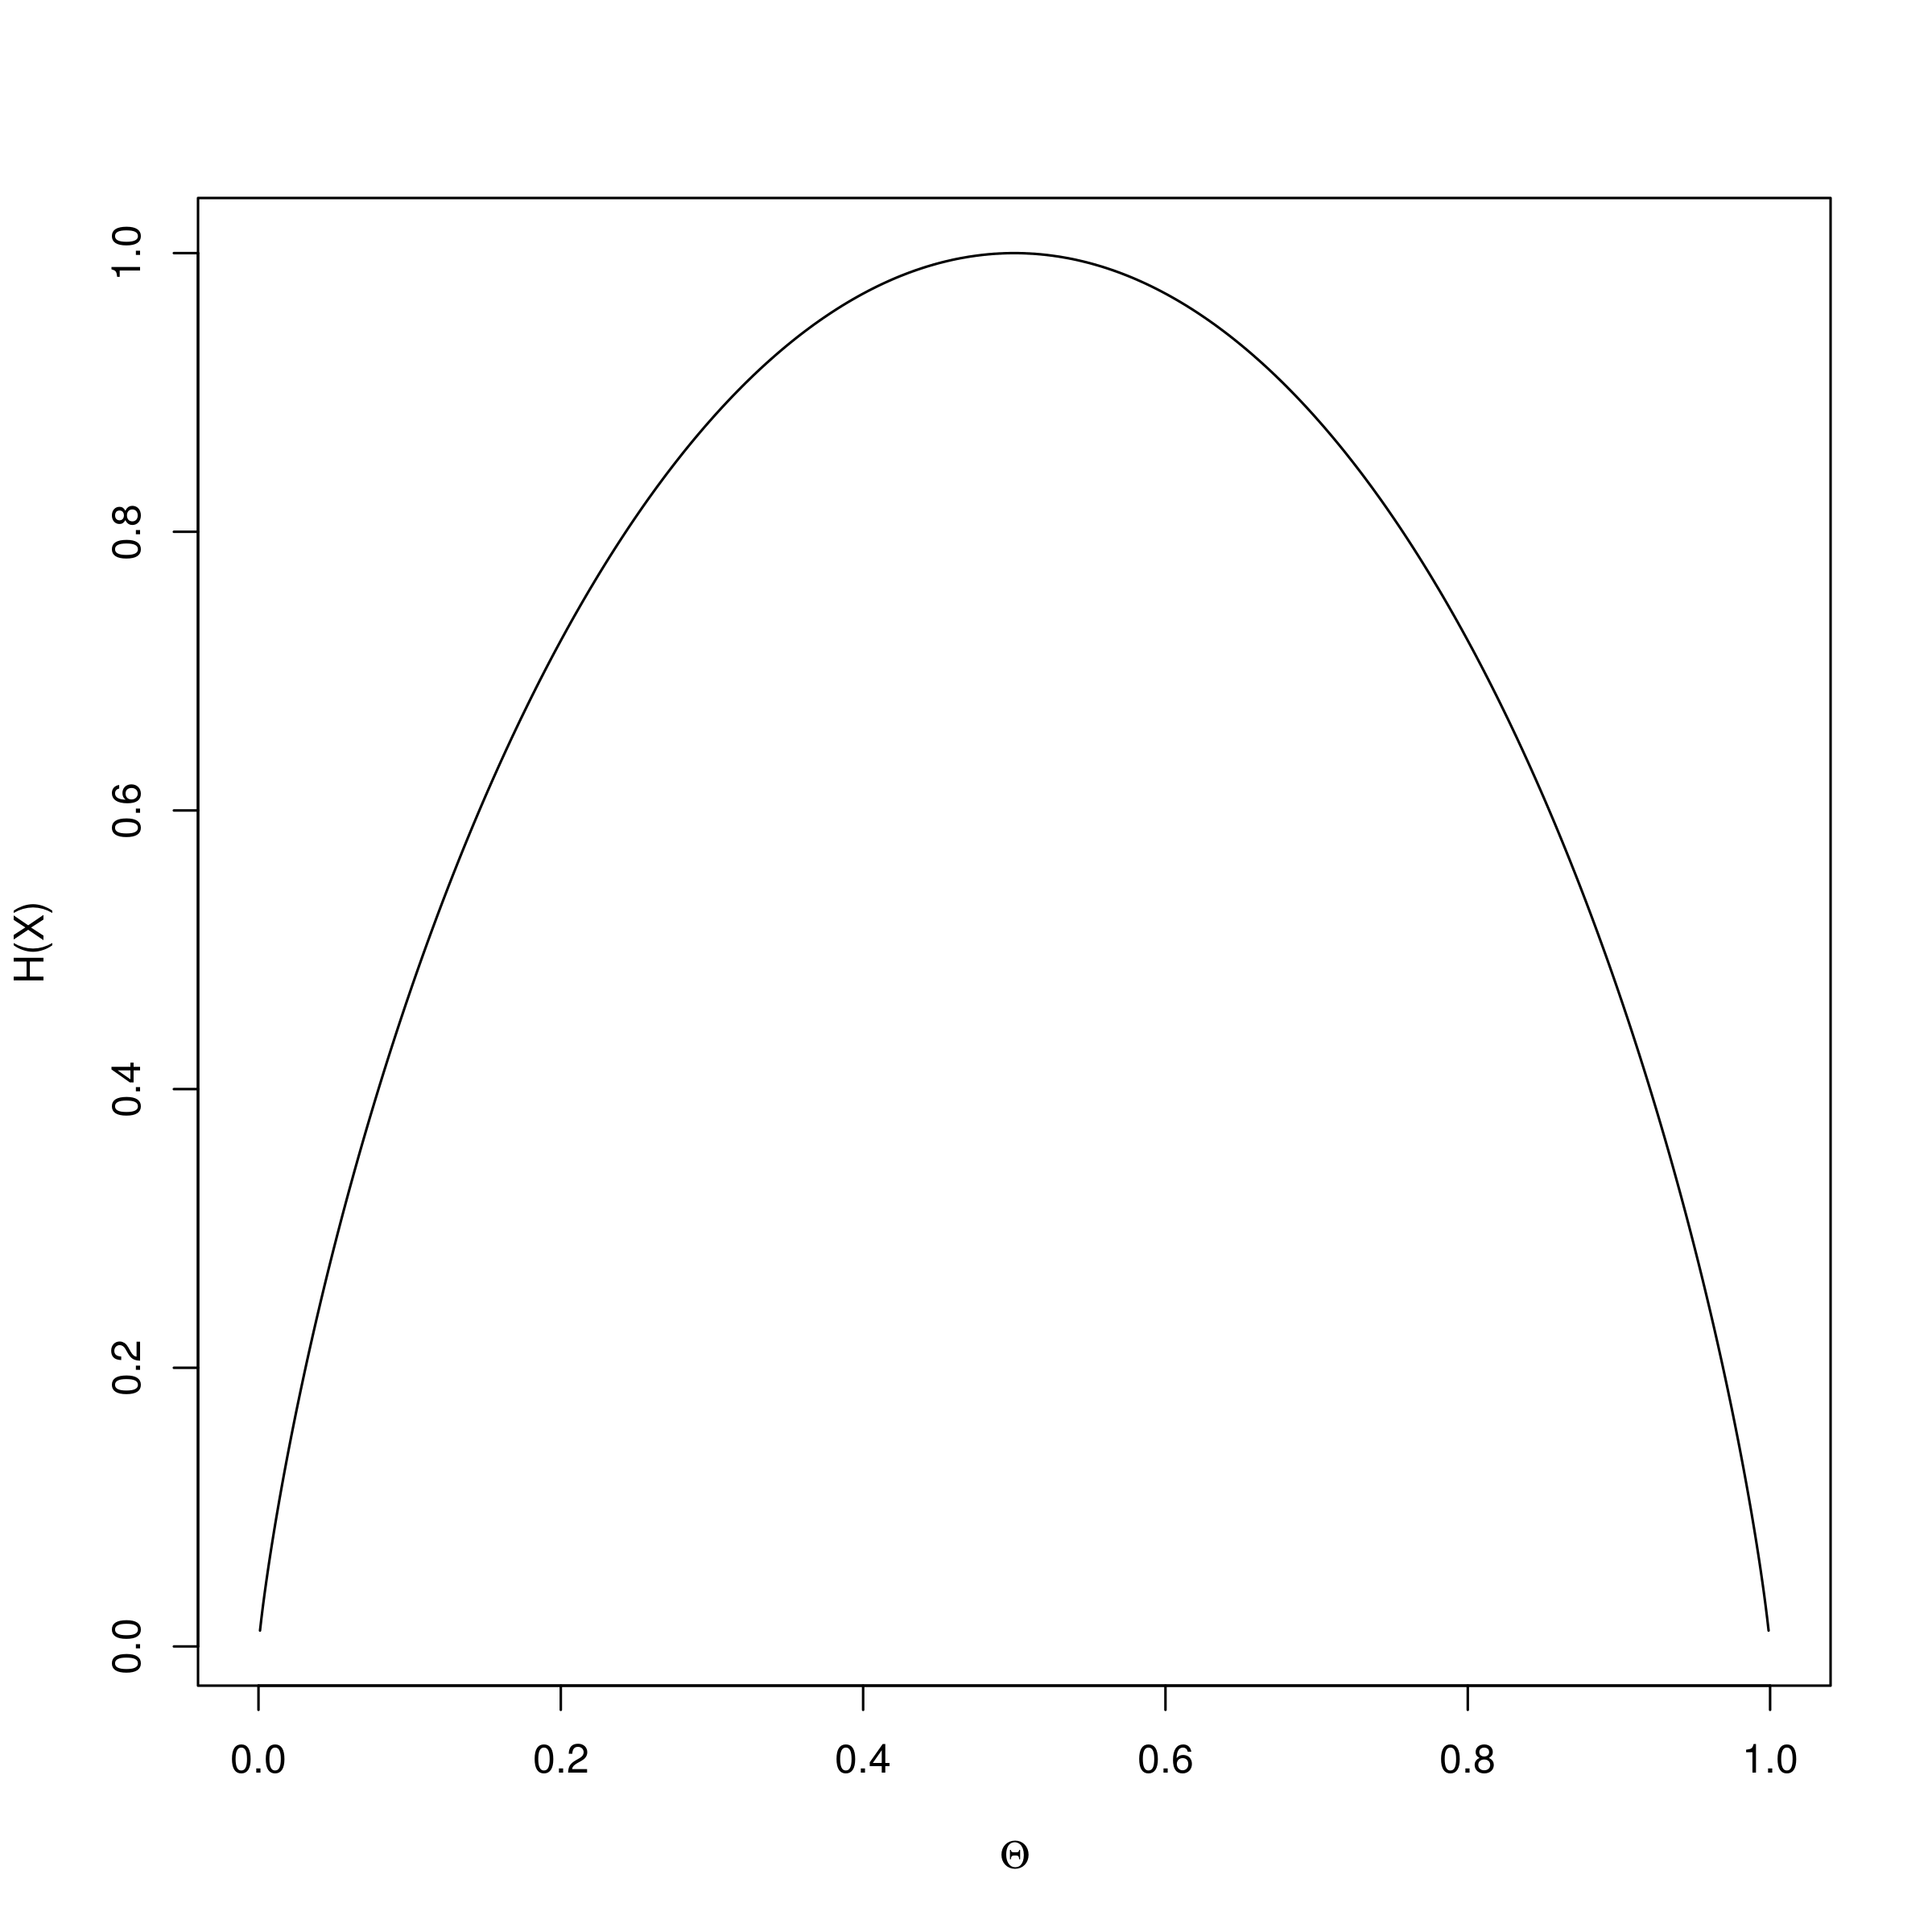
\includegraphics[scale=0.5]{binaryEntropy.png}
\caption{Binary entropy function.}
\label{fig:binaryEntropy}
\end{figure}

From the plot is it also easy to see that entropy is never negative. It holds in general that entropy is non-negative,
because entropy is defined as expectation of surprisal and surprisal is the negative logarithm of probabilities. 
Because $ \log(x) \leq 0 $ for $ x \in (0,1] $, it is clear that $ -\log(x) \geq 0 $ for $ x $ in the same
interval. Notice that from here on we drop the subscript and by convention let $ \log = \log_{2} $.

A standard interpretation of the entropy is that it quantifies uncertainty. As we have pointed out
before, a uniform distribution means that you are most uncertain and
indeed the uniform distribution maximizes the entropy. However, the more choices you have to pick from, the more uncertain you are going to be. 
The entropy function also captures this intuition. Notice that if a discrete distribution is uniform,
all probabilities are $ \frac{1}{|\supp(X)|} $. Clearly, as we increase $ |\supp(X)| $, we decrease the
probabilities. By decreasing the probabilities, we increase their negative logarithms, and hence their
surprisal. Let us make this intuition more formal.

\begin{Theorem}
A discrete RV $ X $ with uniform distribution and support of size $ n $ has entropy
$ H(X) = \log(n) $.
\end{Theorem}

\paragraph{Proof:}
\begin{align}
H(X) &= \underset{x \in \supp(X)}{\sum}-\log(P(X=x))P(X=x) \\
&= \underset{x \in \supp(X)}{\sum}\log(n)P(X=x) = \log(n) \, . ~~~~\square
\end{align}

\begin{Exercise}
You are trying to learn chess and you start by studying where chess grandmasters move their king when it
is positioned in one of the middle fields of the board. The king can move to any of the adjoining 8 fields. Since
you do not know a thing about chess yet, you assume that each move is equally probable. In this situation,
what is the entropy of moving the king?
\end{Exercise}

At the outset of this section we promised you that you could easily transfer results from probability 
theory to information theory. We will not be able to show any kind of linearity for entropy because it contains
log-terms and the logarithm is not linear. We can however find alternative expressions for joint entropy (where 
the joint entropy is simply the entropy of a joint RV). Before we do so, let us also define the notion of 
conditional entropy. We have seen in Section~\ref{sec:jointconditionaldistributions} that $P_{X|Y=y}$ is a valid probability distribution for any $y \in \supp(Y)$ such that $P(Y=y)>0$. Hence, we can also define its conditional entropy.

\begin{Definition}[Conditional Entropy]
For two jointly distributed RVs $ X,Y $ and $y \in \supp(Y)$ such that $P(Y=y)>0$, the conditional entropy of $ X $ given that $ Y=y $ is defined as
$$ H(X|Y=y) := \E_X[-\log_{2}(P(X=x|Y=y))] \, . $$
The conditional entropy of $X$ given $Y$ is defined as
$$ H(X|Y) := \E_Y[ H(X|Y) ] = \sum_{y \in \supp(Y)} P(Y=y) H(X|Y=y) \, .$$
\end{Definition}

With this definition at hand we show that the joint entropy decomposes according to the
chain rule.

\begin{align*}
H(X,Y) &= \underset{\substack{x \in \supp(X)\\y \in \supp(Y)}}{\sum} -\log(P(X=x,Y=y)) \times P(X=x, Y=y) \\
\begin{split}
&= \underset{\substack{x \in \supp(X)\\ y \in \supp(Y)}}{\sum} -\log(P(X=x| Y=y)) \times P(X=x,Y=y) \\ 
&\qquad - \underset{y \in \supp(Y)}{\sum}\log(P(Y=y)) \times \sum_{x \in \supp(X)} P(X=x,Y=y) 
\end{split} \\
\begin{split}
&=\sum_{y \in \supp(Y)} P(Y=y) \times \sum_{x \in \supp(X)} -\log(P(X=x| Y=y)) \times P(X=x|Y=y) \\ &\qquad - \underset{y \in \supp(Y)}{\sum}\log(P(Y=y)) \times P(Y=y)
\end{split} \\
&= H(X|Y) + H(Y)
\end{align*}

\begin{Exercise}
Prove that $ H(X,Y|Z) = H(X|Z) + H(Y|Z) $ if $ X \bot Y|Z $.
\end{Exercise}

Now that we have seen some information-theoretic concepts, you may be happy to hear that there is an information-theoretic interpretation
of EM. This interpretation helps us to get a better intuition for the algorithm. To formulate that interpretation we need
one more concept, however.

\begin{Definition}[Relative Entropy]
The relative entropy of RVs \\ $ X,Y $ with distributions $P_X, P_Y$ and $\supp(X) \subseteq \supp(Y) $ is defined as \chris{I think we should leave out the middle term with the expectation, the notation we are using reaches its limit here...}
$$ D(P_X||P_Y) := \E_{X}}\left[\log \frac{P(X=X)}{P(Y=X)} \right] = \sum_{x \in \supp(X)} P(X=x) \log \frac{P(X=x)}{P(Y=x)} \ . $$
If $ P(X=y) = 0 $ for any $ y \in \supp(Y) $ we define $ D(P_X||P_Y) = \infty $. As with entropy, we often abbreviate $D(P_X||P_Y)$ with  $D(X||Y)$.
\end{Definition}

The relative entropy is commonly known as \textbf{Kullback-Leibler (KL)} divergence. It measures the entropy of $ X $ as scaled to $ Y $. Intuitively,
it gives a measure of how ``far away'' $ P_{X} $ is from $ P_{Y} $. To understand ``far away'', recall that entropy is a measure of uncertainty. The
relative entropy measure the uncertainty that you have about $ P_{X} $ if you know $ P_{Y} $\chris{hard to see why at this point}. This uncertainty is low if both distributions place most
of their mass on the same outcomes. Since $ \log(1) = 0 $ the relative entropy is 0 if $ P_{X} = P_{Y} $.

It is worthwhile to point out the difference between relative and conditional entropy. Conditional entropy is the average entropy of $ X $ given that you
know what value $ Y $ takes on. In the case of relative entropy you do not know the value of $ Y $, only its distribution.

\begin{Exercise}
\philip{We can use this one for homework.} Show that $ D(X,Y|Y) = H(X|Y) $. Furthermore show that $ D(X,Y|Y) = H(X) $ if $ X\bot Y $.
\end{Exercise}

\philip{Include this?}
\section{An Information-theoretic Interpretation of EM}

\section*{Further reading}

At the ILLC, the best place to learn more about information theory is \href{http://homepages.cwi.nl/~schaffne/courses/inftheory/2015/}{Christan Schaffner's}
course that is taught every year. David MacKay also offers \href{http://www.inference.phy.cam.ac.uk/itprnn/book.pdf}{a free book on the subject}. Finally,
Coursera also offers \href{https://www.coursera.org/course/informationtheory}{an online course on information theory}.

To get a better understanding of EM and the other concepts discussed in this script along with some more examples, consult 
\href{http://www.cs.columbia.edu/~mcollins/em.pdf}{Micheal Collins' lecture notes} .

\end{document}



%%% Local Variables:
%%% mode: latex
%%% TeX-master: "chapter6"
%%% End:
